\chapter{Implementação}
\label{sec-implementacao}
\section{introdução}
dar uma introdução aqui

Começamos inicializando o Pygame e definindo o título da janela, criamos três variáveis de controle \textit{home\_open, credits\_open} e \textit{controls\_open} que servem para definir qual aba estará sendo renderizada e três instancias de objetos \textit{home}, \textit{credits} e \textit{controls}  que são os objetos que definem a tela , a variável de controle \textit{home\_open} é inicializada como verdadeiro pois é a tela que será mostrada inicialmente. esse programa fica em um \textit{loop} enquanto captura os eventos e inputs do jogador na tela \textit{home}.
\lstinputlisting[label=lst:main, caption=Main, language=Python, float=htpb]{codigos/main.py}

\newpage
\lstinputlisting[label={lst-home}, caption=Home, language=Python, float=htpb]{codigos/home.py}

Em \textit{home} como mostra a listagem \ref{lst-home} definimos o tamanho da tela que é 1280 x 720, importamos as imagens e áudios que são usados nessa tela, reproduzimos a musica e criamos uma variável \textit{index} que é utilizada para saber qual opção o jogador escolheu, também é guardado as três funções de \textit{callback} \textit{run\_game}, \textit{run\_credits}, \textit{run\_game\_controls} que tem as funções de alterar as variáveis de controle da main para a troca de contexto. Para explicar a função \textit{draw\_menu} é necessário explicar alguns conceitos do pygame, para desenhar imagens em pontos específicos é necessário ter um retângulo associado, esse retângulo representa onde será renderizada a imagem, para esse propósito existe a classe nativa Pygame\textit{Rect}, essa classe também é utilizada para fazer checagem de colisões e a movimentação, sua assinatura é a seguinte.
\begin{itemize}
    \item \textit{\textbf{x:}} posição em x em que sera desenhado;
    \item \textit{\textbf{y:}} posição em y em que sera desenhado;
    \item \textit{\textbf{width:}} largura do retângulo;
    \item \textit{\textbf{height:}} altura do retângulo;
\end{itemize}

Normalmente não queremos jogar com personagem que seja um retângulo, ou interagir com quadrados ou círculos, então associamos uma imagem a esse objeto retângulo, o método \textit{pygame.image.load} carrega uma imagem para o Pygame passando o arquivo como parâmetro e retorna um objeto \textit{Surface} essa classe Surface é utilizada para a representação das imagens no Pygame.
\begin{figure}[h!]
    \centering
    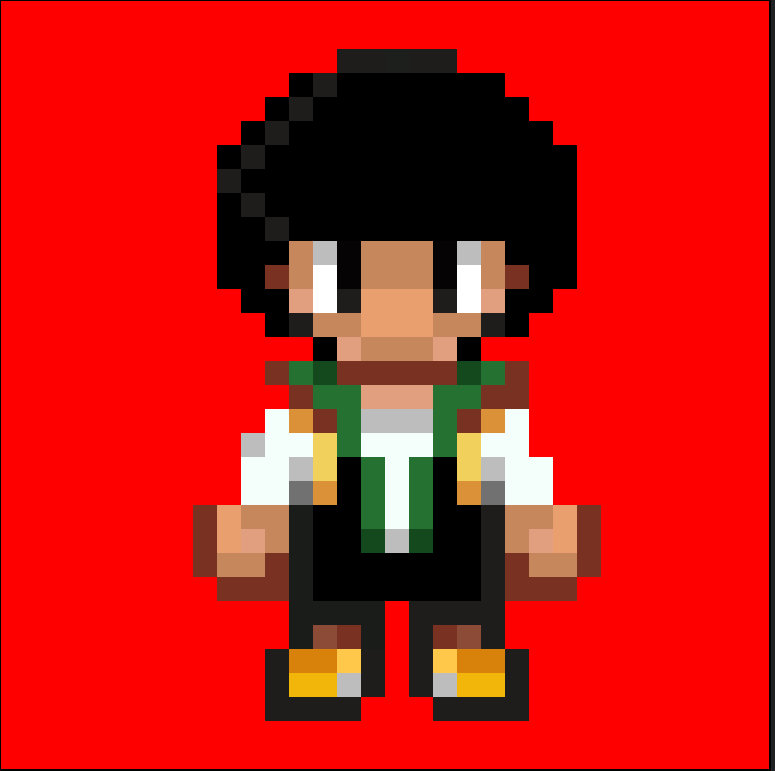
\includegraphics[width=0.5\linewidth]{figuras/player.png}
    \caption{Exemplo de Retângulo Associado a Imagem do Personagem Principal}
    \label{fig:player}
\end{figure}

Com essas informações podemos explicar a função \textit{draw\_menu} ela responsável por desenhar as informações dessa tela de home, os retângulos de seleção da tela e a imagem de fundo, para causar o efeito de iluminação sobre os retângulos é feito o uso do método \textit{blit} do pygame, essa função tem a seguinte assinatura.
\begin{itemize}
    \item \textit{\textbf{source}:} a imagem \textit{Surface} a ser desenhada sobre o \textit{Surface} atual;
    \item \textit{\textbf{dest (opcional):}} posição onde será desenhado a imagem, sendo o padrão o canto superior esquerdo (0, 0)
    \item \textit{\textbf{area (opcional):}} a delimitação da área retangular para desenhar.
    \item \textit{\textbf{special\_flags (opcional:}} controla como as cores do da imagem serão combinadas com a Superfície.
\end{itemize}
É graças ao quarto parâmetro \textit{special\_flags} que é possível causar esse efeito, usando a \textit{flag} \textit{BLEND\_RGB\_ADD } misturamos as cores RGB da mesma imagem com o fundo branco e é adicionado os canais de cor de origem aos canais de cor de destino.

\begin{figure}[h!]
    \centering
    
\includegraphics[width=1\linewidth]{figuras/blit_example.png}
    \caption{Exemplo de Sobreposição de Imagens com o Método \textit{blit}}
    \label{fig:blit-example}
\end{figure}

A operação de \% (resto da divisão) é feita sobre o index para garantir que a opção selecionada pelo jogador seja somente uma das opções definidas, a variável \textit{new\_rect} que tem armazenada um retângulo que será a área a ser desenhada na tela um retângulo em python é representado pela classe nativa \textit{Rect} ela permite a representação desses retângulos na tela seus parâmetros são

Todos os retângulos de seleção da tela inicial tem o tamanho fixo 123 x 90, o que muda é a posição que ele sera desenhado, que varia de acordo com o index selecionado, tendo uma checagem para o programa saber qual imagem será desenhada.

\newpage
\lstinputlisting[label=lst:game, caption=Game, language=Python, float=htpb]{codigos/game.py}
No Pygame um \textit{sprite} pode ser representado com a classe nativa \textit{Sprite} herdar essa classe base e adicionar os atributos e métodos que nos interessa é muito útil como por exemplo se somado a classe \textit{container Groups} nesta é possível adicionar Sprites que podem ser criados para comportamentos específicos, como na instanciação da classe game que a listagem \ref{lst:game} mostra, essa é a classe responsável por inicializar todas as variáveis assets e chamar as funções principais do programa \textit{import\_assets} que carrega para o Pygame todos os assets do jogo e \textit{setup} que carrega e inicializa o mapa, as variáveis com o prefixo \textit{tint} são para o controle do efeito de transição (linhas 9 a 14), também é feito a inicialização do inventário (linhas 45 e 46) e do computador (linhas 47 e 48)  ela é chamada após o jogador escolher a opção \textit{new} no menu inicial, na linha (9) é criado o objeto \textit{all\_sprites} esse objeto é usado como a câmera do jogador, a classe \textit{AllSprites} herda \textit{Group} e nele estão todos os sprites do jogo, nas linhas (10) a (14) da listagem \ref{lst:game} são criadas 5 variáveis que são do tipo Group, cada uma dessas variáveis tem um propósito especificado a seguir
\begin{itemize}
    \item \textit{\textbf{collision\_sprites: }}Nessa variável estão todos os sprites colidíveis do jogo;
    \item \textit{\textbf{character\_sprites: }}Essa variável contém todos os sprites de personagens do game;
    \item \textit{\textbf{transition\_sprites: }}Aqui contém todos os sprites de colisão;
    \item \textit{\textbf{dialogs\_sprites: }}Todos os sprites que geram uma caixa de diálogo estão aqui;
    \item \textit{\textbf{interaction\_sprites: }}Neste estão presentes todos os objetos do jogo que são interativos;
\end{itemize}

import assets
\lstinputlisting[label=lst-import-assets, caption=Import Assets, language=Python, float=htpb]{codigos/import_assets.py}
\newpage
Essa função carrega todos os assets do jogo e retorna um dicionário para cada tipo de \textit{frames} sendo eles
\begin{itemize}
    \item \textit{\textbf{tmx\_maps: }}contém todos os mapas;
    \item \textit{\textbf{overworld\_frames: }}contém os assets de personagem, e do lago;
    \item \textit{\textbf{fonts: }}contém todos as fontes do game;
    \item \textit{\textbf{interface\_frames: }}contém todos os assets relacionado a interface do jogo;
\end{itemize}


setup
\lstinputlisting[label=lst-setup caption=Setup, language=Python, float=htpb]{codigos/setup.py}
\newpage
Função responsável por limpar os \textit{sprites} do mapa anterior após uma transição e carregar os \textit{sprites} do mapa atual, bem como alocar todos os \textit{sprites} aos seus respectivos grupos
\begin{table}[h!]
	\caption{Tabela especificando os tipos de \textit{sprites} presentes em Super Labes World}
	\label{tbl-especificacao-sprites}
	\centering
	\renewcommand{\arraystretch}{3}
	\begin{small}
		\begin{tabular}{ | p{37mm} | p{23mm}  | p{52mm} | p{30mm} | }\hline \rowcolor{MidnightBlue}
			\centering{\textbf{Classe}} & \centering{\textbf{Camadas}} & \textbf{Descrição} & \textbf{Grupos} \\\hline		
                \centering{\textit{Sprite}} & \centering{\textit{Terrain, Terrain Top, Terrain Objects}} & {Classe com os tiles da camada mais baixa sem colisões} & {\textit{all\_sprites}} \\\hline
                \centering{\textit{AnimatedSprite}} & \centering{\textit{Lake, Lake Edges}} & {Classe com tiles animados do lago sem colisão} & {\textit{all\_sprites}} \\\hline			
                \centering{\textit{CollidableSprite}} & \centering{\textit{Objects}} & {Classe com os sprites de objetos do jogo com colisão} & {\textit{all\_sprites, collision\_sprites}} \\\hline		
                \centering{\textit{InteractiveSprite}} & \centering{\textit{Interactive Objects}} & {Classe com os sprites com interação com colisão} & {\textit{all\_sprites, collision\_sprites, interactive\_sprites}} \\\hline	
                \centering{\textit{CollisionSprite}} & \centering{\textit{Collisions}} & {Classe com as colisões sem uma imagem} & {\textit{collision\_sprites}} \\\hline		
                \centering{\textit{CollidableDialogSprite}} & \centering{\textit{Dialogs}} & {Classe com os sprites de diálogo} & {\textit{dialog\_sprites}} \\\hline		
                \centering{\textit{TransitionSprite}} & \centering{\textit{Transitions}} & {Classe que armazena os sprites de transição sem imagem} & {\textit{transition\_sprites}} \\\hline		
                \centering{\textit{Player}} & \centering{\textit{Entities}} & {Classe do jogador principal} & {\textit{all\_sprites}} \\\hline		
                \centering{\textit{Character}} & \centering{\textit{Entities}} & {Classe para representar as entidades de personagens do jogo} & {\textit{all\_sprites, collision\_sprites, characters\_sprites}} \\\hline		
		\end{tabular}
	\end{small}
\end{table}

Os personagens são adicionados pelo ferramenta Tiled citado na seção \ref{sec:tiled} para carregar os personagems e o jogador é criado um retangulo no programa com as seguintes propriedades.
\begin{itemize}
    \item \textbf{\textit{character\_id: }}É com essa variavel que lidamos para definir qual dos sprites será mostrado nesse personagem ;
    \item \textbf{\textit{direction: }}Define qual é a posição inicial do jogador ;
    \item \textbf{\textit{pos: }}Mapa anterior que o player estava antes da transição, é necessário por que todo mapa tem pelo menos dois \textit{players} devido a transição de ida e de volta essa variável então é usada para o Pygame saber qual das posições desenhar o jogador ;
\end{itemize}

\begin{figure}[h!]
    \centering
    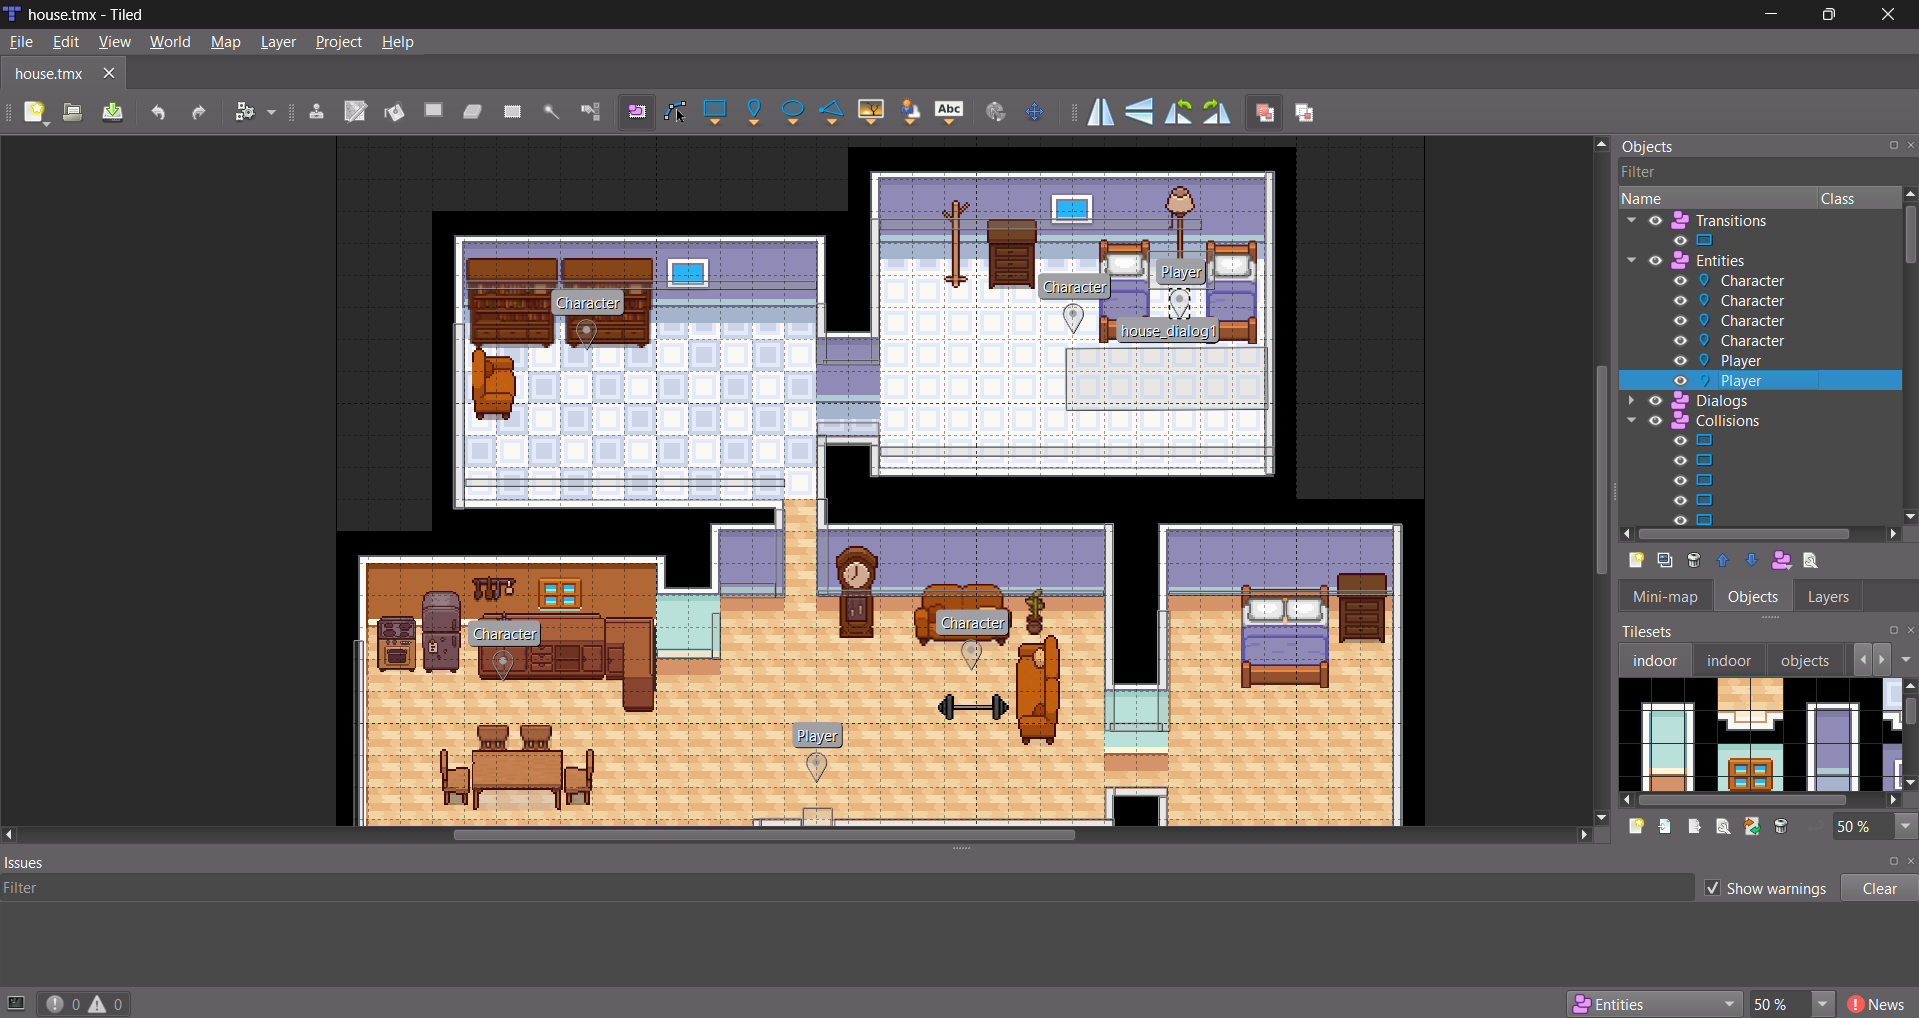
\includegraphics[width=1\linewidth]{figuras/tiled-house.png}
    \caption{Posicionamento de Objetos no Software Tiled }
    \label{fig:tiled-house}
\end{figure}

\begin{figure}[h!]
    \centering
    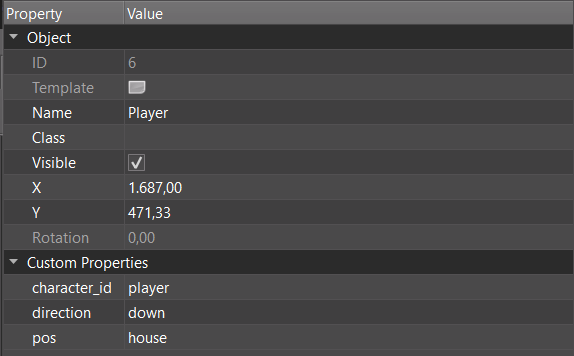
\includegraphics[width=1\linewidth]{figuras/tiled-player-properties.png}
    \caption{Propriedades da Entidade Player no Tiled}
    \label{fig:tiled-player-propertiesl}
\end{figure}


% game loop
\lstinputlisting[label=lst-game-loop, caption=Main, language=Python, float=htpb]{codigos/game_loop.py}
\newpage
Essa é a função com o loop principal do jogo, preenchemos o fundo do mapa com preto, definimos o delta time como já explicado na seção \ref{sec:delta-time} e [e feita a verificação de evento fechar a janela como dito na seção \ref{sec:pygame-ce} a partir da linha 14 começa a lógica do jogo
\begin{itemize}
    \item Linha (14) função responsável por tratar a entrada de teclado do jogador será explicada com mais detalhes na listagem \ref{lst-input};
    \item Linha (15) função responsável por verificar se o jogador colidiu com um \textit{sprite} de transição quando for o caso chama a função \textit{setup} com os parâmetros do mapa a ser transicionado;
    \item Linha (16) função responsável por verificar se o jogador colidiu com alguma caixa de diálogo, se sim então chamando a função para criar o diálogo com a mensagem; 
    \item Linha (17) função responsável por atualizar todos os sprites da tela; 
    \item Linha (20) função responsável por ser a câmera do jogador; 
\end{itemize}

\textit{overlays} ou sobreposição 
(linhas 23 a 28) da listagem \ref{lst-game-loop} durante o jogo normal todas 
\begin{itemize}
    \item \textit{\textbf{dialog\_open: }} verdadeiro quando o jogador aperta \textit{"backspace"} próximo a uma personagem do jogo, então troca de contexto do \textit{loop} principal para o \textit{loop} da classe \textit{Dialog};
    \item \textit{\textbf{inventory\_open: }}verdadeiro caso de o jogador aperte a tecla "i", troca o contexto do \textit{loop} principal para o \textit{loop} da classe \textit{Inventory}; 
    \item \textit{\textbf{computer\_open: }} verdadeiro quando o jogador aperta "\textit{backspace}" próximo a \textit{InteractiveObject} com o \textit{"item\_id"} = \textit{computer}, troca de contexto do \textit{loop} principal para o \textit{loop} da classe \textit{Computer};
    \item \textit{\textbf{battle\_open: }}  verdadeiro quando o jogador o jogador responde sim para um desafio de um personagem com questões, nesse caso troca-se de contexto para a batalha;
    \item \textit{\textbf{choose\_dialog\_open: }} verdadeiro ao fim de um diálogo de um personagem que contém questões e que não foi derrotado;

\end{itemize}



% input
\lstinputlisting[label=lst-input, caption=Input, language=Python, float=htpb]{codigos/input.py}

\clearpage

Outras informações adicionais, 
para resolver o problema do retângulo do personagem ser associado a imagem como visto na figura \ref{fig:player} existe um método para lidar com isso \textit{inflate} essa função diminui se passado valores negativos ou aumenta caso contrário o tamanho de retângulo, a listagem figura \ref{lst-player-hitbox} a figura \ref{fig:player-hitbox} simula o resultado diminuindo a largura pela metade e 60 píxels de altura.

\begin{lstlisting}[language=Python,breaklines, caption= Uso da Função Inflate, label= lst-player-hitbox]
self.hitbox = self.rect.inflate(-self.rect.width / 2, -60)
\end{lstlisting}
\begin{figure}[h!]
    \centering
    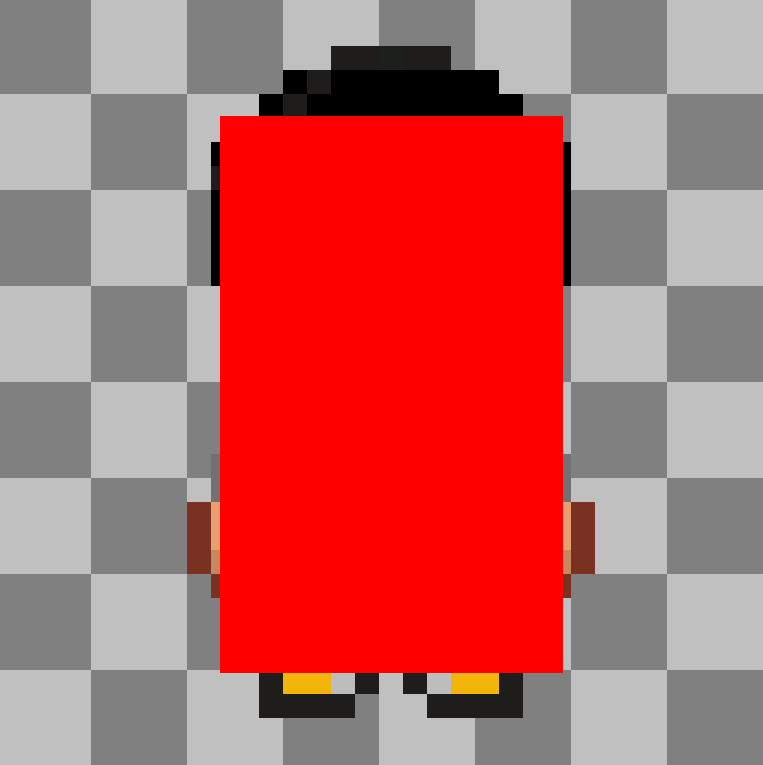
\includegraphics[width=0.5\linewidth]{figuras/player-hitbox.png}
    \caption{\textit{Hitbox} do Personagem Principal}
    \label{fig:player-hitbox}
\end{figure}



